\begin{enumerate}
	\item If two lines are perpendicular to one another then the relation between their slopes $m_{1}$ and $m_{2}$ is:
		\begin{enumerate}
			\item $m_{1} = m_{2}$
			\item $m_{1} = \frac{1}{m_{2}}$
			\item $m_{1} = -m_{2}$
			\item $m_{1} \times m_{2} = -1$
		\end{enumerate}
	\item The coordinates of the point $P(-3,5)$ on reflecting on the $x$-axis are:
		\begin{enumerate}
			\item $(3, 5)$
			\item $(-3, -5)$
			\item $(3, -5)$
			\item $(-3, 5)$
		\end{enumerate}
	\item $A(1, 4), B(4, 1)$ and $C(x, 4)$ are the vertices of $\bigtriangleup ABC$. If the centroid of the triangle is $G(4, 3)$ then $x$ is equal to:
		\begin{enumerate}
			\item $2$
			\item $1$
			\item $7$
			\item $4$
		\end{enumerate}
	\item Find $'a'$, if $A(2a + 2, 3$, $B(7,4)$ ad $C(2a +5, 2)$ are collinear.
	\item Find a point $P$ which divides internally the line segment joining the points $A(-3, 9)$ and $B(1, -3)$ in the ratio $1:3$.
	\item Use a graph paper for this question. Take $2 cm = 1$ unit along both the axes\\
		\begin{enumerate}
			\item Plot the points $A(0, 4), B(2, 2), C(5,2)$ and $D(4,0)$. $E(0, 0)$ is the origin.
			\item Reflect $B, C, D$ on the $y$-axis and name them as $B', C', D'$ respectively.
			\item Join the points $ABCDD'C'B'$ and $A$ in order and give a geometrical name to the closed figure.
		\end{enumerate}
	\item Find the equation of a line parallel to the line $2x + y - 7 = 0$ and passi    ng through the intersection of the lines $x + y- 4 =0$ and $2x - y =8$.
	\item Line $AB$ is perpendicular to $CD$. Coordinates of $B, C and D$ are respectively $(4, 0), (0, -1)$ and $(4,3)$.
		\begin{figure}[h]
			\centering
			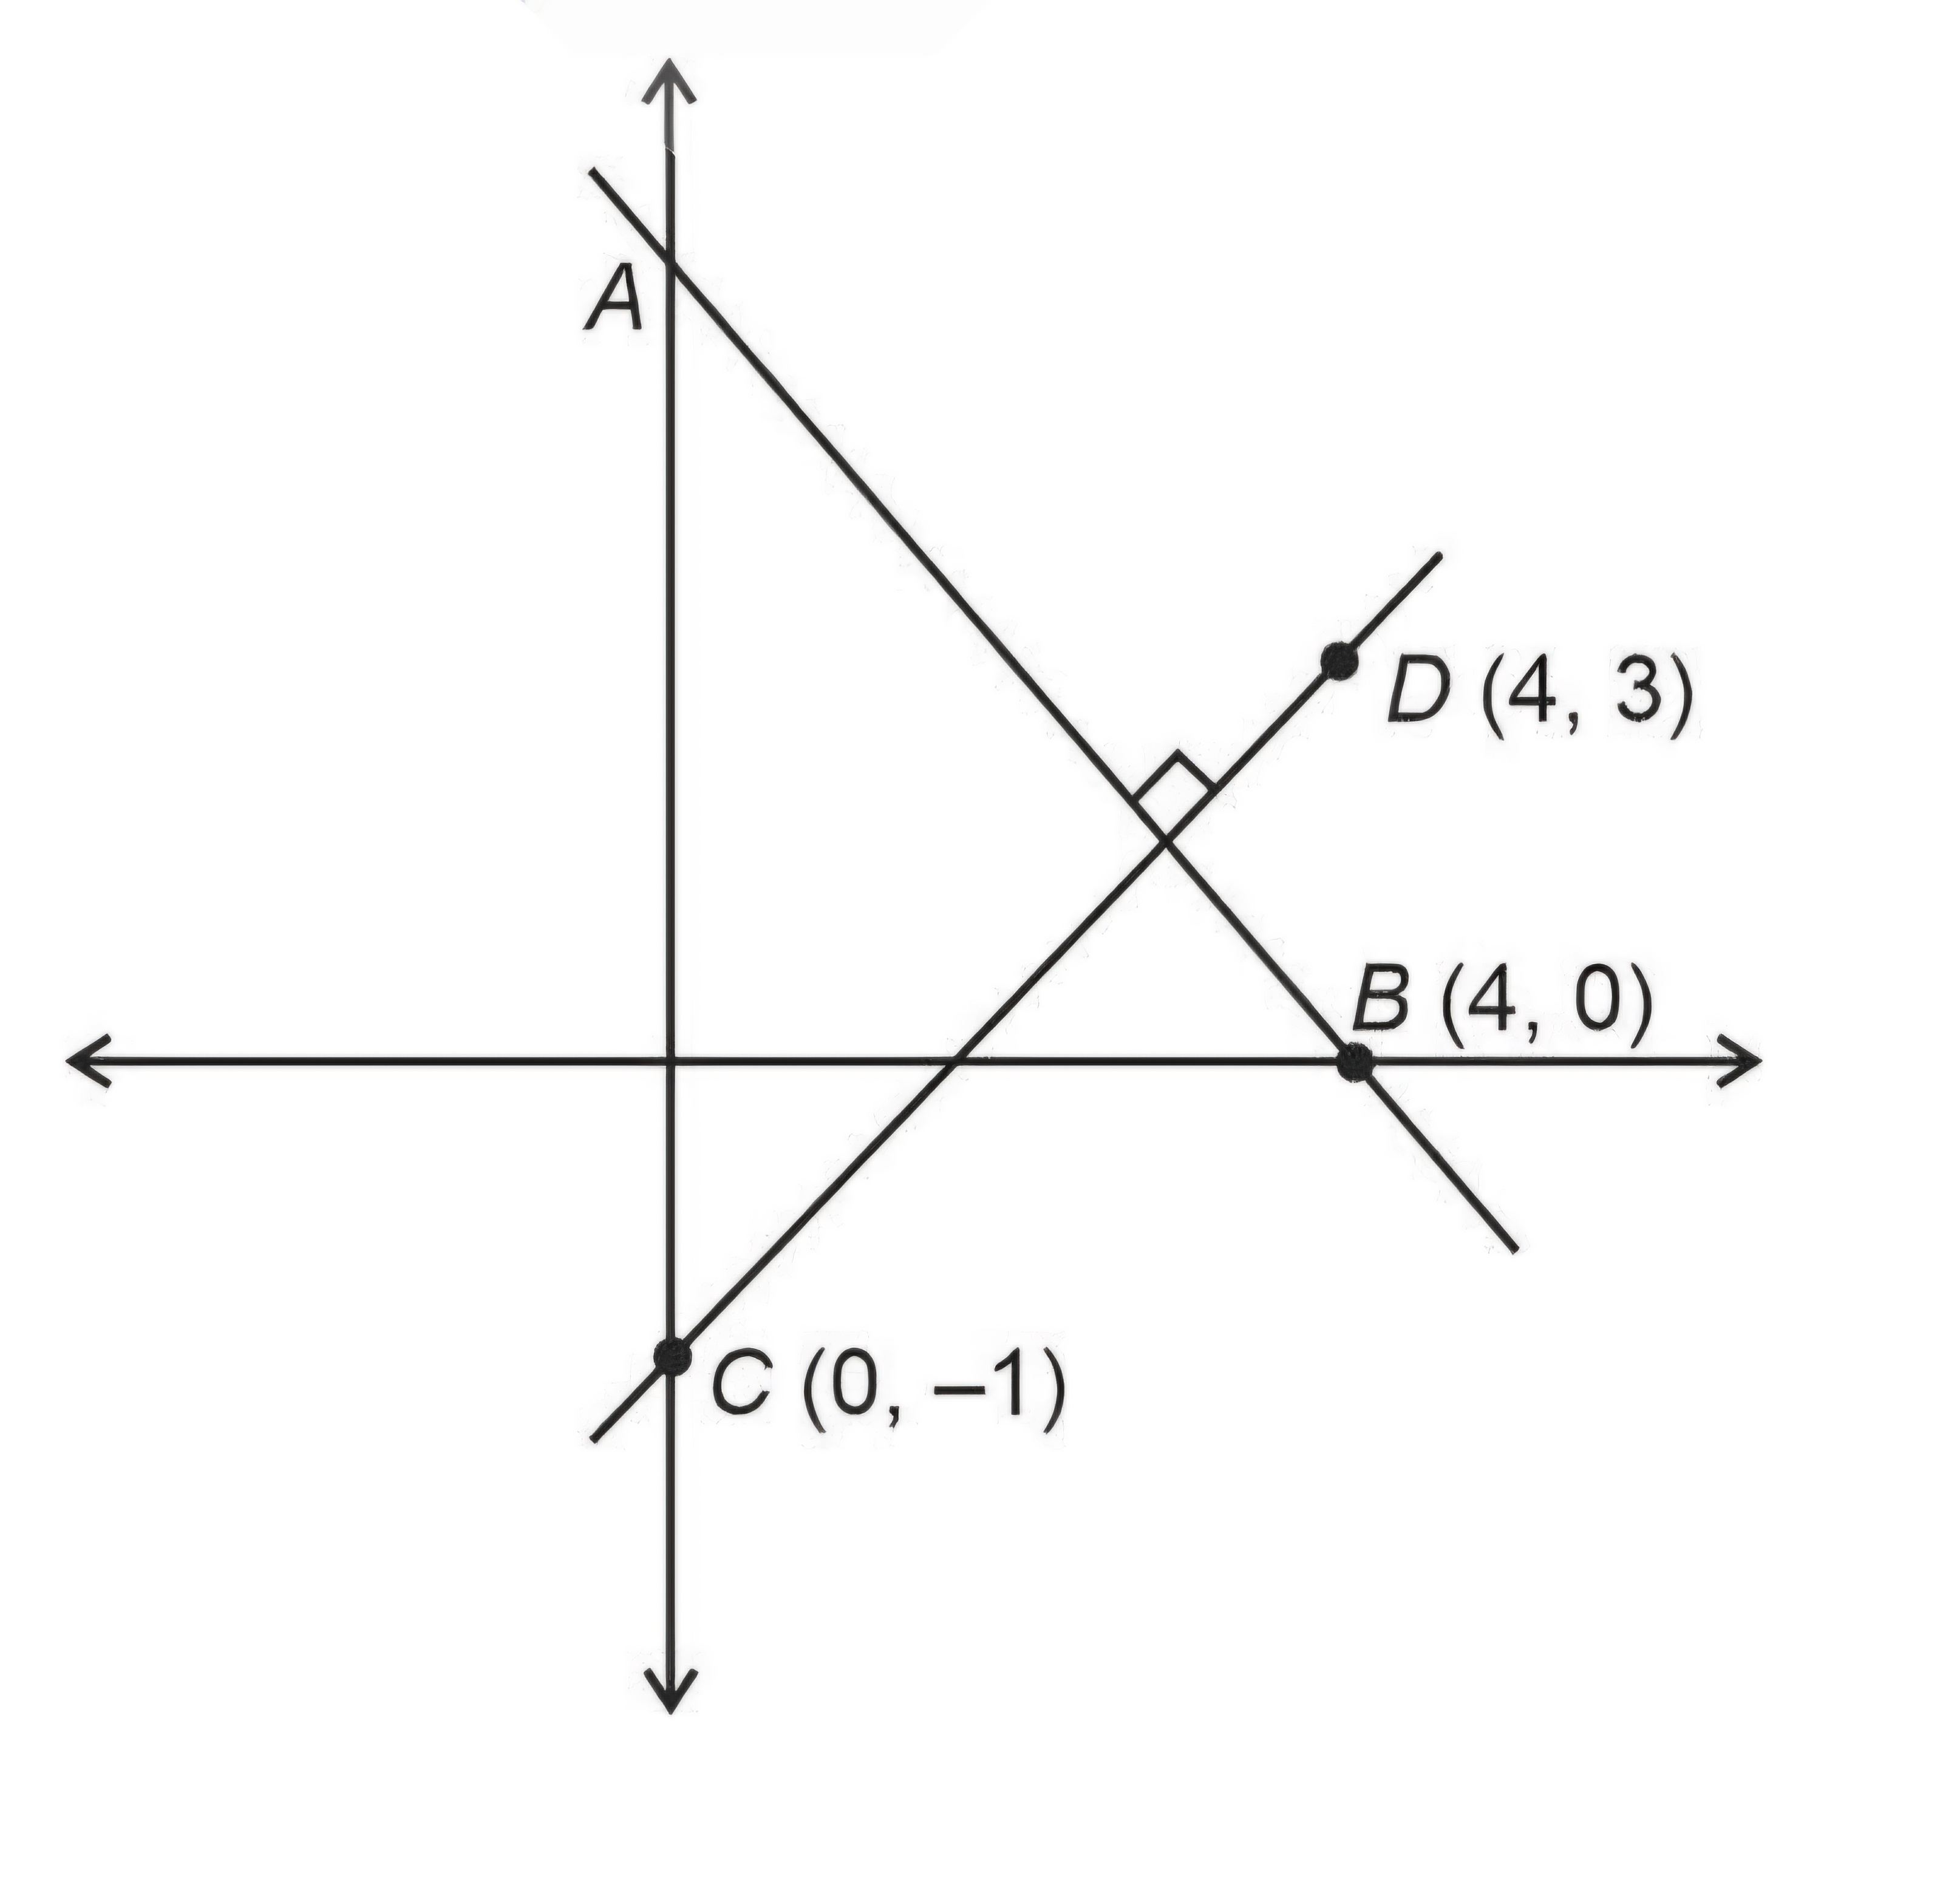
\includegraphics[width=\columnwidth]{figs/img6.jpg}
			\caption{}
			\label{figure}
		\end{figure}
		Find:
		\begin{enumerate}
			\item Slope of $CD$
			\item Equation of $AB$
		\end{enumerate}
\end{enumerate}
